%%
%% This is file `sample-sigconf.tex',
%% generated with the docstrip utility.
%%
%% The original source files were:
%%
%% samples.dtx  (with options: `sigconf')
%% 
%% IMPORTANT NOTICE:
%% 
%% For the copyright see the source file.
%% 
%% Any modified versions of this file must be renamed
%% with new filenames distinct from sample-sigconf.tex.
%% 
%% For distribution of the original source see the terms
%% for copying and modification in the file samples.dtx.
%% 
%% This generated file may be distributed as long as the
%% original source files, as listed above, are part of the
%% same distribution. (The sources need not necessarily be
%% in the same archive or directory.)
%%
%% The first command in your LaTeX source must be the \documentclass command.
\documentclass[sigconf]{acmart}
% \usepackage[mediumspace,mediumqspace,Grey,squaren]{SIunits}
\usepackage{siunitx}
\usepackage[ruled,vlined]{algorithm2e}
\usepackage{graphicx} %package to manage images
\graphicspath{ {./res/} }
%%
%% \BibTeX command to typeset BibTeX logo in the docs
\AtBeginDocument{%
  \providecommand\BibTeX{{%
    \normalfont B\kern-0.5em{\scshape i\kern-0.25em b}\kern-0.8em\TeX}}}

%% Rights management information.  This information is sent to you
%% when you complete the rights form.  These commands have SAMPLE
%% values in them; it is your responsibility as an author to replace
%% the commands and values with those provided to you when you
%% complete the rights form.
\setcopyright{acmcopyright}
\copyrightyear{2018}
\acmYear{2018}
\acmDOI{10.1145/1122445.1122456}

%% These commands are for a PROCEEDINGS abstract or paper.
\acmConference[Woodstock '18]{Woodstock '18: ACM Symposium on Neural
  Gaze Detection}{June 03--05, 2018}{Woodstock, NY}
\acmBooktitle{Woodstock '18: ACM Symposium on Neural Gaze Detection,
  June 03--05, 2018, Woodstock, NY}
\acmPrice{15.00}
\acmISBN{978-1-4503-XXXX-X/18/06}


%%
%% Submission ID.
%% Use this when submitting an article to a sponsored event. You'll
%% receive a unique submission ID from the organizers
%% of the event, and this ID should be used as the parameter to this command.
%%\acmSubmissionID{123-A56-BU3}

%%
%% The majority of ACM publications use numbered citations and
%% references.  The command \citestyle{authoryear} switches to the
%% "author year" style.
%%
%% If you are preparing content for an event
%% sponsored by ACM SIGGRAPH, you must use the "author year" style of
%% citations and references.
%% Uncommenting
%% the next command will enable that style.
%%\citestyle{acmauthoryear}

%%
%% end of the preamble, start of the body of the document source.
\begin{document}

%%
%% The "title" command has an optional parameter,
%% allowing the author to define a "short title" to be used in page headers.
\title{Paper Title}

%%
%% The "author" command and its associated commands are used to define
%% the authors and their affiliations.
%% Of note is the shared affiliation of the first two authors, and the
%% "authornote" and "authornotemark" commands
%% used to denote shared contribution to the research.
\author{Author 1}
\email{trovato@corporation.com}
\orcid{1234-5678-9012}
\author{G.K.M. Tobin}
\authornotemark[1]
\email{webmaster@marysville-ohio.com}
\affiliation{%
  \institution{Institute for Clarity in Documentation}
  \streetaddress{P.O. Box 1212}
  \city{Dublin}
  \state{Ohio}
  \postcode{43017-6221}
}

\author{Author 2}
\affiliation{%
  \institution{The Th{\o}rv{\"a}ld Group}
  \streetaddress{1 Th{\o}rv{\"a}ld Circle}
  \city{Hekla}
  \country{Iceland}}
\email{larst@affiliation.org}

%%
%% By default, the full list of authors will be used in the page
%% headers. Often, this list is too long, and will overlap
%% other information printed in the page headers. This command allows
%% the author to define a more concise list
%% of authors' names for this purpose.
\renewcommand{\shortauthors}{Trovato and Tobin, et al.}

%%
%% The abstract is a short summary of the work to be presented in the
%% article.
\begin{abstract}
 Spin-Transfer Torque Random Access Memory (STT-RAM) has emerged as a promising alternative to SRAM based on-chip caches across all levels of cache hierarchy due to its low leakage power, high density and non-volatility. But the high write energy and write latency of STT-RAM is still an hindrance to its wide scale adoption. One popular approach towards mitigating these overheads is to relax STT-RAM's retention time, which in turn reduces the high write latency and energy. However, to prevent the cache data blocks from expiring prematurely some refresh scheme is needed which has its own overheads impacting the performance and energy of the cache.
 
 Towards minimising these refresh overheads, in this paper we propose a method to reduce the number of dynamic refreshes needed to maintain data integrity. Leveraging the reduced cell area of STT-RAM we create a Refresh Confidence table which is used to learn interleaving access duration of the blocks using the cache access pattern and is used to decide if a block needs to be refreshed. Eliminating unnecessary refreshes helps to reduce the memory access stalls required when the data is being refreshed as well reduce dynamic energy. Our experiments shows that the proposed method can reduce the refreshes by 25\%, refresh energy by 84\% and dynamic energy by 9\% for STT-RAM based caches.

\end{abstract}

%%
%% The code below is generated by the tool at http://dl.acm.org/ccs.cfm.
%% Please copy and paste the code instead of the example below.
%%
\begin{CCSXML}
<ccs2012>
<concept>
<concept_id>10010520.10010521.10010528.10010536</concept_id>
<concept_desc>Computer systems organization~Multicore architectures</concept_desc>
<concept_significance>500</concept_significance>
</concept>
</ccs2012>
\end{CCSXML}

\ccsdesc[500]{Computer systems organization~Multicore architectures\vspace{1.5em}}



%%
%% Keywords. The author(s) should pick words that accurately describe
%% the work being presented. Separate the keywords with commas.
\keywords{STT-RAM, Refresh Energy, Cache, Retention Time, Non-Volatile Memory, Write Latency, Write Energy}

%% A "teaser" image appears between the author and affiliation
%% information and the body of the document, and typically spans the
%% page.

% \begin{teaserfigure}
%   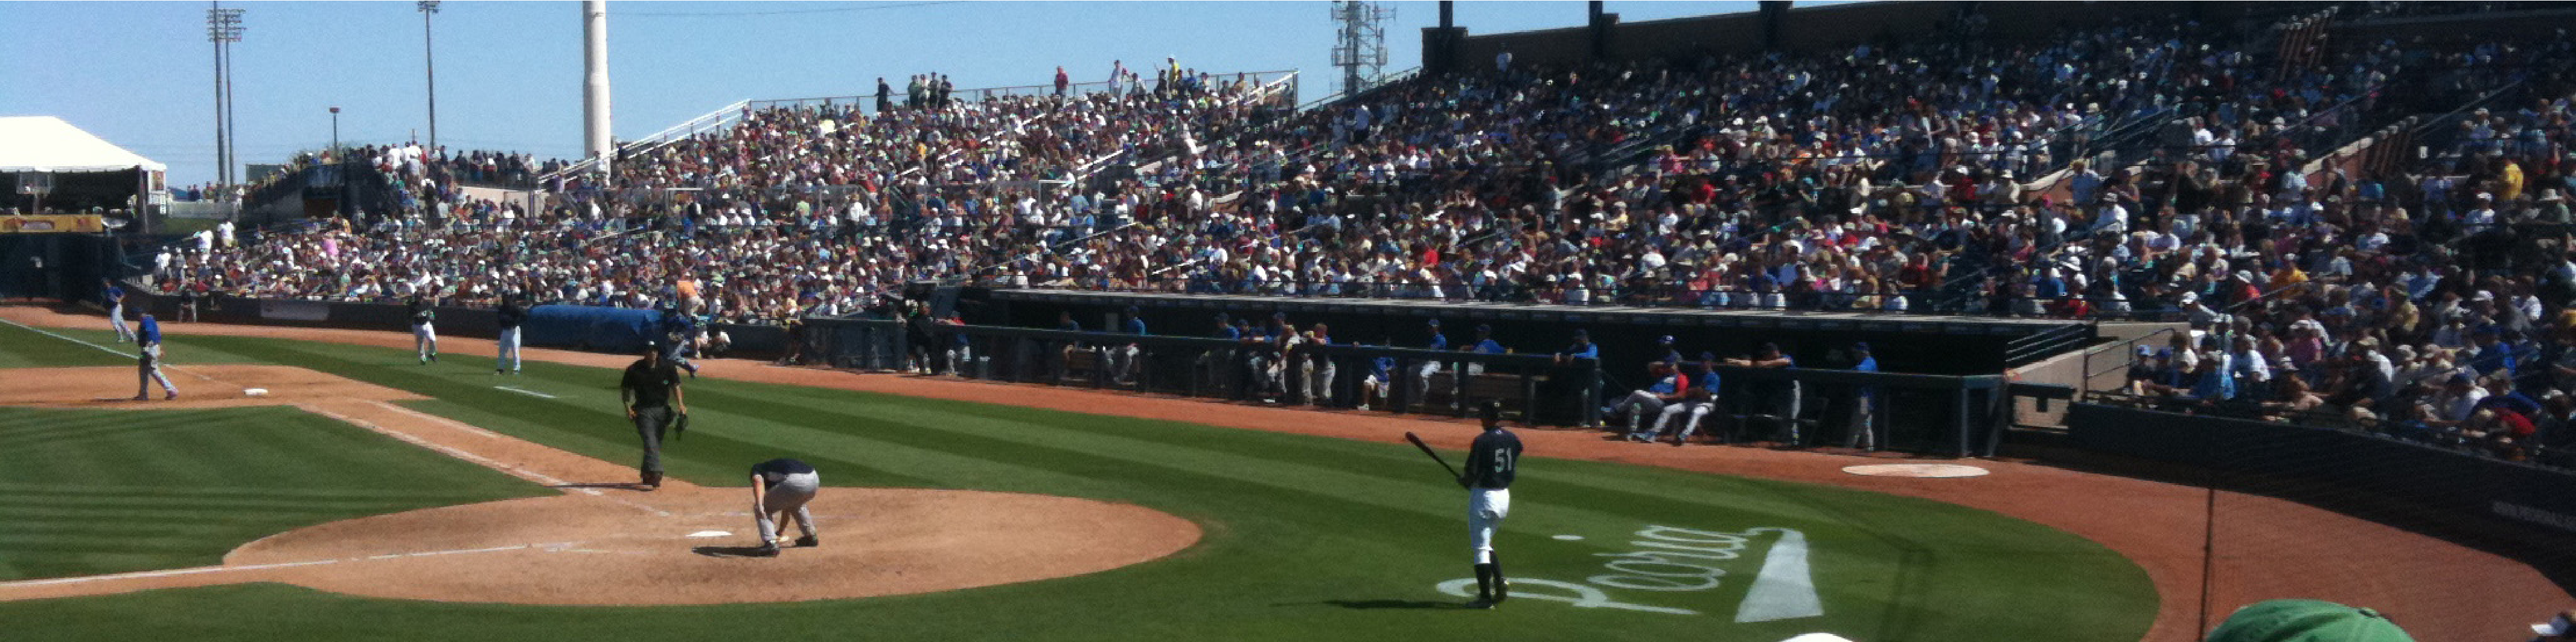
\includegraphics[width=\textwidth]{sampleteaser}
%   \caption{Seattle Mariners at Spring Training, 2010.}
%   \Description{Enjoying the baseball game from the third-base
%   seats. Ichiro Suzuki preparing to bat.}
%   \label{fig:teaser}
% \end{teaserfigure}

%%
%% This command processes the author and affiliation and title
%% information and builds the first part of the formatted document.
\maketitle

\section{Introduction}
The growing popularity of multi-core architectures have also concomitantly stressed the demand for larger and more optimized caches to bridge the performance gap between processor and memory. This has led to a gradual increase in cache sizes across all the hierarchies over the years to reduce performance penalty incurred on cache misses. However, with increasing capacity the leakage power of SRAM based caches have started to dominate the total power consumption of the processor. To mitigate this overhead the Spin-Transfer Torque RAM (STT-RAM) is emerging as one of the most viable alternative to replace SRAM. STT-RAM has this potential due to its non-volatility, low leakage power, high cell density and competitive read latency. However, the high latency and energy associated with write operations in STT-RAM incur major overheads that needs to be mitigated in order to make their performance competitive to SRAM.
    
    A promising approach to reduce the write energy and latency is to relax
the retention time of STT-RAM\cite{smullen}. The retention time indicates the duration for which the data is retained in the memory without any power, which is generally about 10 years for STT-RAM. However, this long retention time is over-provisioned for the requirements of the L1 as well as LLC cache blocks. Analysis done in previous work\cite{liang} for L1 Cache shows that revival time of cache blocks are typically in \textit{\SI{}{\micro\second}} range. Thus reducing the retention time serves as a viable trade off to counter balance the high write energy and latency of SRAM.

A few prior works have explored the benefits of relaxed retention time designs\cite{cache_revive}, \cite{compiler}, \cite{smullen}, \cite{sun}. Most of them use some form of  \textit{dynamic refresh scheme} to prevent premature expiry of cache blocks. These dynamic refreshes have overheads of their own impacting energy and performance as pointed out in \cite{compiler}, limiting the  optimization that could be achieved by STT-RAM based cache. There hasn't been a lot of focus into reducing the refresh overheads as reduction in leakage energy dominates the net energy savings while comparing with an SRAM based cache. But these refresh energy can go as high as -- of total dynamic energy in a few PARSEC benchmarks.The work in \cite{compiler} has tried to reduce the \textit{active refreshes} by modifying data access pattern while compilation but it incurs associated overheads in terms of extra circuits and compilation time. In \cite{cache_revive} the refreshes are reduced by using an extra buffer to revive top half of MRU blocks but this incurs a substantial energy overhead due to the buffer's leakage energy\cite{mirror_cache}.


Our work is motivated by \cite{rrip} where \textit{Re-Reference Interval} of every cache block is learnt to modify the cache replacement policy. In this paper we propose a mechanism to minimize the \textit{active refreshes} required to maintain cache data integrity by using the
\begin{figure}[]
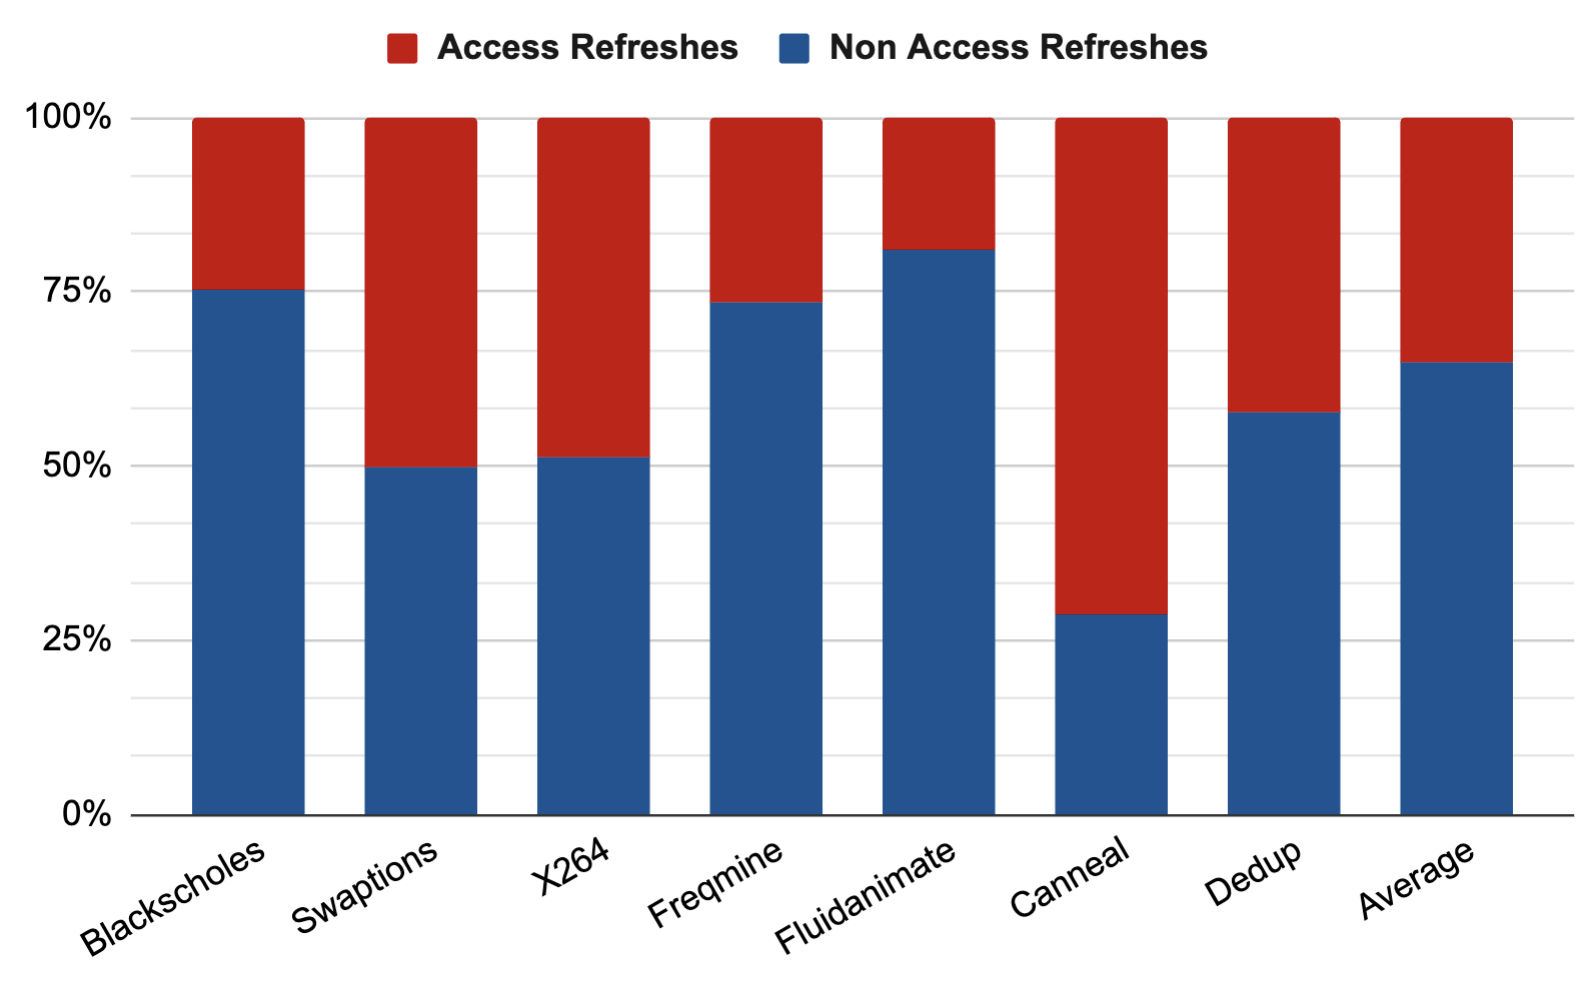
\includegraphics[width=\columnwidth]{res/ref_percentage.png}
\caption{Percentage of Access and Non-Access refreshes for various benchmarks}
\end{figure}
access pattern of in-memory data blocks to decide whether to refresh a block when it reaches the end of its retention time, with an optimization goal to not incur significant cache miss penalty due to reducing the refreshes. Our major contributions are as follows:
\begin{itemize}
  \item As per our knowledge, this is the first work to explore cache access pattern to reduce the number of dynamic refreshes.
  \item We propose a low overhead mechanism to dynamically learn the refresh requirements of every cache block and use it reduce non-necessary refreshes.
  \item We compare our method with both SRAM and STT-RAM based methods to investigate its potential. Experiments show that we are able to reduce the number of refreshes by 25\% and 70\% as compared to CacheRevive and MirrorCache respectively. The effective reduction in dynamic energy was 9\% and 4\% respectively.
\end{itemize}

The reset of the paper is organised as follows: Background and Related works are presented in section II. The proposed Learning based Refresh Reduction Technique in described in section III. Section IV describes the experimental methodology and Section V discusses the experimental results. Section VI concludes the paper.

\section{BACKGROUND AND RELATED WORK}

The structure of STT-RAM and the existing methods to reduce the inherent retention time of STT-RAM by modifying its thermal barrier have been detailed in the previous works \cite{cache_revive}, \cite{scaling_roadmap}. In this section we some summarise some of the prior work related to dynamic refresh schemes that provides the background for our work. 

\subsection{Refresh schemes}

The relaxation of retention time in STT-RAM have been show to significantly reduce the write energy and latency to values competitive to SRAM. To prevent the premature data loss due to the reduced retention time from affecting the cache miss rate several refresh schemes have been proposed. The refresh scheme proposed in \cite{sun} uses state based counters to monitor the expiry status of the blocks. When the counter saturates to its final state the blocks are refreshed and this keeps on continuing for every block till it is either invalidated or evicted from cache. This method incurs significant energy overheads as the number of refreshes are very large. As as improvement over the aforementioned refresh scheme, Jog et al. \cite{cache_revive} proposed \textit{cache revive}. This method refreshes only the most recently used blocks by copying the expiring blocks into a refresh buffer and then again moving it back to its original place in the cache. Utilizing the high density of STT-RAM, this scheme is able to bridge the latency issues associated with STT-RAM by increasing the cache capacity by 4x. The proposed methods in \cite{compiler} uses compiler based code optimization to reduce the refresh count. This is achieved by rearranging the data layout at compile time so that the data blocks are passively refreshes by interleaving write operations. But since the re-arrangement is done at compile time, any scope for runtime optimization is not possible in this method.

All the variants of \textit{dynamic refresh schemes} mentioned above require an additional buffer to temporarily store the expiring blocks before writing them back to the cache. Thus a single refresh operation requires two reads and two writes to move the data back and forth. The energy overheads associated with these refresh operations can amount to substantial portion of cache energy consumption \cite{compiler}. \textit{MirrorCache}\cite{mirror_cache} is one of the recent works that addresses the issue by modifying how refreshes are done. Leveraging the high density of STT-RAM, MirrorCache uses two identical cache segments called the main and auxiliary segment. On a blocks expiry instead of copying the data in the refresh buffer, it is copied into the auxiliary segment and subsequent access to those blocks are redirected there. When the block expires in auxiliary segment, it copied back to main segment. Thus a block keeps moving on between the two segments until it gets invalidated or replaced. This eliminates the need for an external refresh buffer and the overhead of leakage energy associated with it. The energy optimization of this method is solely based on the reduction in static energy while there still exists an opportunity to reduce the dynamic energy incurred in refresh operations. This will be our focus for optimization which is discussed ahead.

\subsection{Motivation for proposed scheme}

To illustrate the scale of refreshed blocks in different retention time regions, we analysed the number of refreshes done by MirrorCache in \SI{100}{\micro\second} and \SI{1}{\milli\second} retention time caches on PARSEC 2.1 benchmark suite \cite{parsec}. These two specific retention time were chosen because the revival time analysis done by previous work \cite{liang} for L1 cache shows it be in \sisetup{detect-all = true} \textit{\SI{}{\micro\second}} range. \sisetup{detect-none = true}
Figure 1 shows the number of refreshes for various benchmarks on 32 KB L1 cache.
It also shows the portion of those refreshes that leads to no read or write access till the next refresh is needed. The average portion of \textit{non-access} refreshes is about 60\% of total refreshes. We aim to reduce these refreshes without affecting the cache misses significantly. This optimization can help to reduce the caches dynamic energy and performance by reducing the stalls required due to cache being busy in refresh operations. 


\section{PROPOSED Methodology}
This section describes our proposed policy that reduces the number of dynamic refreshes by using a block's access pattern. As mentioned in the previous section, our method focuses on those refreshes that lead to no subsequent access from cache so that they can be prevented from being refreshed without incurring significant degradation on miss rate. We also monitor the performance of our refresh decision module during runtime so that any dynamic changes in data access pattern can be adapted into. Further on we discusses the architectural changes and learning algorithm to do the same.

\subsection{Cache Architecture}
Figure 2 illustrates the proposed architecture. To track the expiry status of the cache blocks we use \textit{monitor counters} associated individually with every block, similar to the work in \cite{sun}. The clock period of the monitor counter is lesser than the cache retention time by a factor of \textit{N}, where \textit{N} is the number of states in monitor counter determined by its number of bits. When the counter reaches its penultimate state, refresh process for that block is initiated so that there exists ample time to complete the refresh before data loss. Any write access to the blocks in between the states resets the counters to its initial state. We have used 2 bits per monitor counter as it gives acceptable trade-off between performance and overheads.

To eliminate the requirement of an highly associative refresh buffer and multiple read and writes per refresh, we use an auxiliary segment to refresh the blocks similar to \cite{mirror_cache}. The tag data is not duplicated for auxiliary segment but the access to data blocks are served from the segment where that block is stored. A single bit status array is used with every block to indicate its current position between main and auxiliary segment. This amounts to a status array size of 512 bit for 32 KB cache. The status array is implemented with the same retention time as data cache because on a refresh to the data block, the status bit needs to flipped which consequently refreshes the data. Apart from this the cache also contains valid and dirty bits for each element as it is with almost all of the state-of-the-art architectures.

The refresh optimization module is the main novelty of our method. It contains a directly mapped table with same number of entries as the number of logical blocks in the cache. This is used to learn and store the \textit{Refresh Confidence} for the residing cache blocks. Refresh confidence is a value assigned to every cache block which is an indirect measure of the confidence of the decision to refresh a block. There exists a fixed one-to-one mapping between the logical cache blocks and table entries. Each entry in table persists till its corresponding block in the cache in overwritten with a different tag block otherwise it is reused for the subsequent accesses by the block with the same tag. This cuts shorts the learning time for the recurring block as the confidence learnt from its previous live time can be directly used to make refresh decisions. A directly mapped table is used to reduce the search overhead of a higher associative version, even though the latter can increase the hit rate in refresh confidence table. To assist with the learning process, each entry in table contains : 1-bit access counter to determine if the block is accessed after the previous refresh, 1-bit status to determine if the block has been refreshed, 4-bit refresh confidence counter and the tag of the block making each entry of 25 bits size. Every refresh request triggered by the monitor counter upon reaching their penultimate stage goes through the refresh optimization module where the refresh confidence entry is used to determine to allow or deny that refresh. This decision is made by comparing the block's learnt confidence with cache's optimization parameter which separately determined using the dynamic cache miss rate.

\begin{figure}[tp]
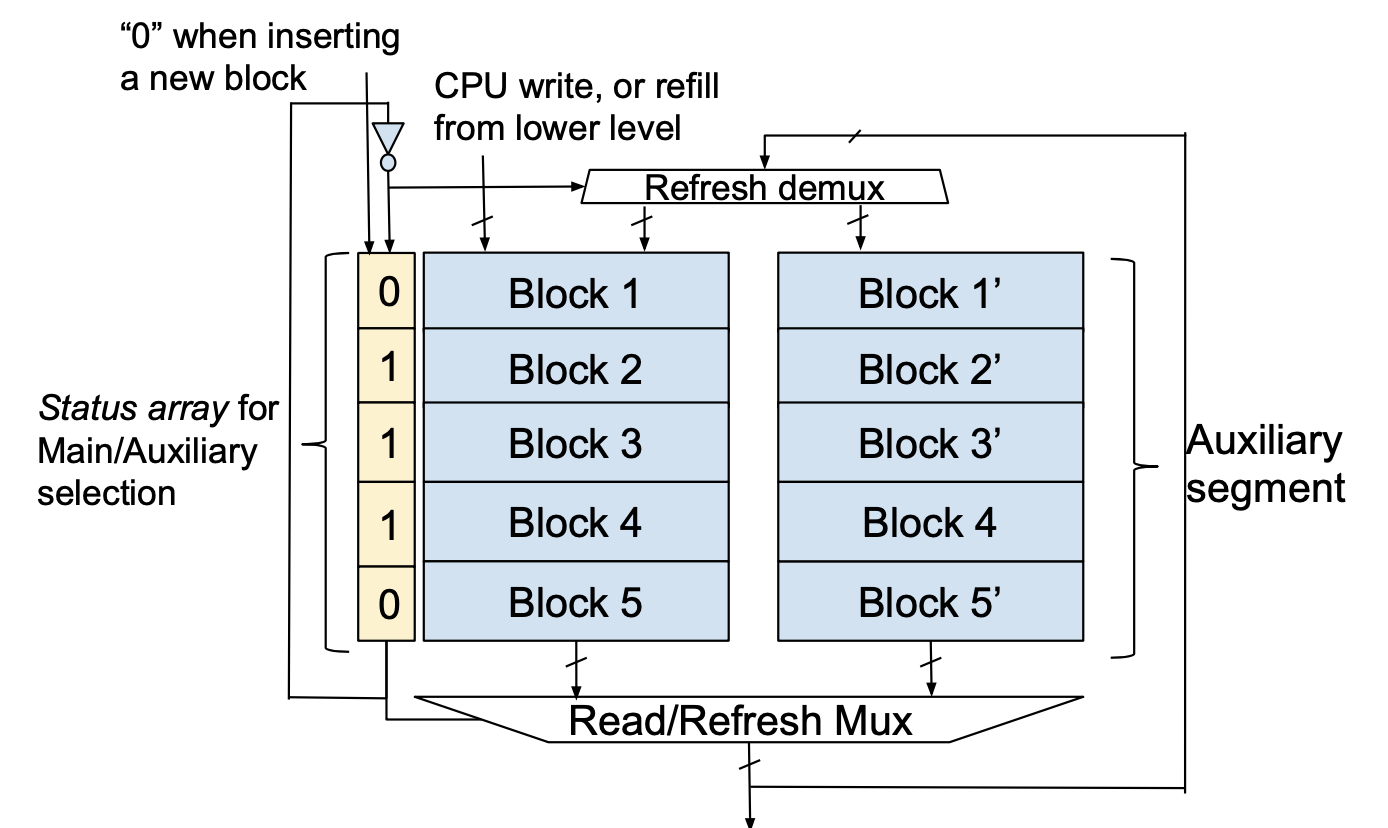
\includegraphics[width=\columnwidth]{res/architecture.png}
\caption{Replace this with own architecture}
\end{figure}

\subsection{Learning the Refresh Confidence}

We have tried to formulate the method to learn the refresh confidence for the blocks using an approach on the lines of \textit{Reinforcement Learning} in which
the state of the agent(status of the cache blocks) changes by the actions (decision to refresh or evict) and the actions are awarded positively or negatively (increasing or decreasing the refresh confidence of the block). 

When a block is brought in the cache for the first time, there is no entry corresponding to it in the refresh confidence table. So upon retention time expiry, its MRU position is used to initialize the entry and decide on its refresh. If the expiring block is among the top 2 MRU blocks, it is refreshed and its entry is initialized with a value of 1 to capture the state that block was recently used and might be reused again otherwise the entry is initialized with 0. On subsequent accesses to the same block, the refresh confidence value can be modified in the following ways:
\begin{itemize}
    \item \textit{\textbf{Cache hit}}: On receiving a cache hit if there exists an entry corresponding to that tag in the confidence table, the value is \textit{increased by 1}. This increment allows to capture recurring accesses to the same block before their actual invalidation due to cache replacement policies because confidence table entries are not evicted if their corresponding data block is invalidated due to retention time expiry. So if a block receives multiple accesses during its retention time period or upon its revival through refresh, its refresh confidence would have been increased accordingly to favor a refresh on expiry.

    \item \textit{\textbf{Cache miss}}: In a relaxed retention time STT-RAM, cache misses can be also due blocks retention time expiry apart from capacity misses and replacement policy invalidation. So the potential benefit of a refresh on a particular block can be estimated by a cache miss if the miss can be directly related to that block not being refreshed on expiry. This is used in the learning algorithm to modify the confidence value. On a miss when an entry for that tag exists in refresh confidence table, the value is \textit{increased} by 1. As an entry still exists in the confidence table but the data block in not in cache, it can be concluded that the previous miss was due to not refreshing the block on expiry, therefore more bias towards refresh can be beneficial for this case.
    
    \item \textit{\textbf{Cache expiry}}: When a block is about to expire, the refresh confidence is \textit{decreased by 0.25} if the block has not been accessed even once. This is done to penalize the last refresh because it didn't amount to any cache hits. Since there can be multiple refreshes between a two consecutive access to a block, the decreasing factor is taken less than the factor by which the value is incremented. This allows the algorithm to wait for multiple \textit{non-access refreshes} before it becomes the major deciding factor for a blocks refresh confidence.
\end{itemize}

\begin{algorithm}[tp]
\SetAlgoLined
 initialization\;
 \While{While condition}{
  instructions\;
  \eIf{condition}{
   instructions1\;
   instructions2\;
   }{
   instructions3\;
  }
 }
 \caption{How to write algorithms}
\end{algorithm}

Figure 3 illustrates the learning algorithm. Using the aforementioned logic, we experimented with different factors to increase and decrease the confidence and found the that 1 and 0.25 gave the best results. With each block having its own refresh confidence, we find the overall threshold at the cache level through a tuning process by starting the application's execution with an initial value of 1 and then increasing it till the cache miss-rate degradation stays under 5\% of the \textit{baseline value}. Baseline value is the minimum miss-rate observed during the tuning process. Once the cache threshold value is tuned, the execution continues with that value till the observed miss-rate stays under 5\% of baseline miss-rate otherwise the tuning process starts again. This dynamic tuning process allows the cache refresh threshold to adjust to changes in the data access pattern. We experimented with a tuning interval of 10 million instruction to give enough time to the new threshold value to affect the refresh process, but this can be decreased further to learn the final threshold value sooner. 



\subsection{Hardware Overhead}
The additional hardware required for this method are: \textit{monitor counters, refresh confidence table} and \textit{auxiliary cache segment}. Each monitor counter has 4 states, which requires 2 bits per counter. With 64B block size, a 32 KB cache has 512 monitor counters which constitutes 0.39\% area overhead. Similarly, with 25 bits per entry the refresh confidence table constitutes 4.9\% area overhead and the auxiliary segment is the same size as that of data cache. But all these area overhead are very easily manageable due the STT-RAM being 3-9 times denser than SRAM \cite{sun}, \cite{cache_revive}. As these units use reduced retention time STT-RAM leakage power is insignificant.

\begin{table*}[t]
\centering
\caption{Cache parameters of STT-RAM with different retention time}
\label{Table:1}
 \begin{tabular} {p{0.2\textwidth}||>{\centering}p{0.2\textwidth}|>{\centering}p{0.2\textwidth}|>{\centering\arraybackslash} p{0.2\textwidth}}
 \hline
%   Col1 & Col2 & Col2 & Col3 \\ [0.5ex] 
 Cache Configuration & \multicolumn{3}{c}{STT-RAM: 32KB, 64B line size, 4-way; Buffer: 1KB} \\ [0.5ex] 
 \hline\hline
 Memory Type & STT-RAM-\SI{100}{\micro\second} & STT-RAM-\SI{1}{\milli\second} & STT-RAM Buffer \\ 
 \hline
 Write Energy per access & \SI{0.095}{\nano\joule} & \SI{0.107}{\nano\joule} & \SI{0.156}{\nano\joule} \\
 \hline
 Hit Energy per access & \SI{0.3}{\nano\joule} & \SI{0.3}{\nano\joule} & \SI{1.089}{\nano\joule} \\
 \hline
 Write Latency (cycles) & 2 & 2 & 1 \\
 \hline
 Hit Latency (cycles) & 3 & 4 & 1 \\ [1ex] 
 \hline
\end{tabular}
\end{table*}


\begin{figure}[th]
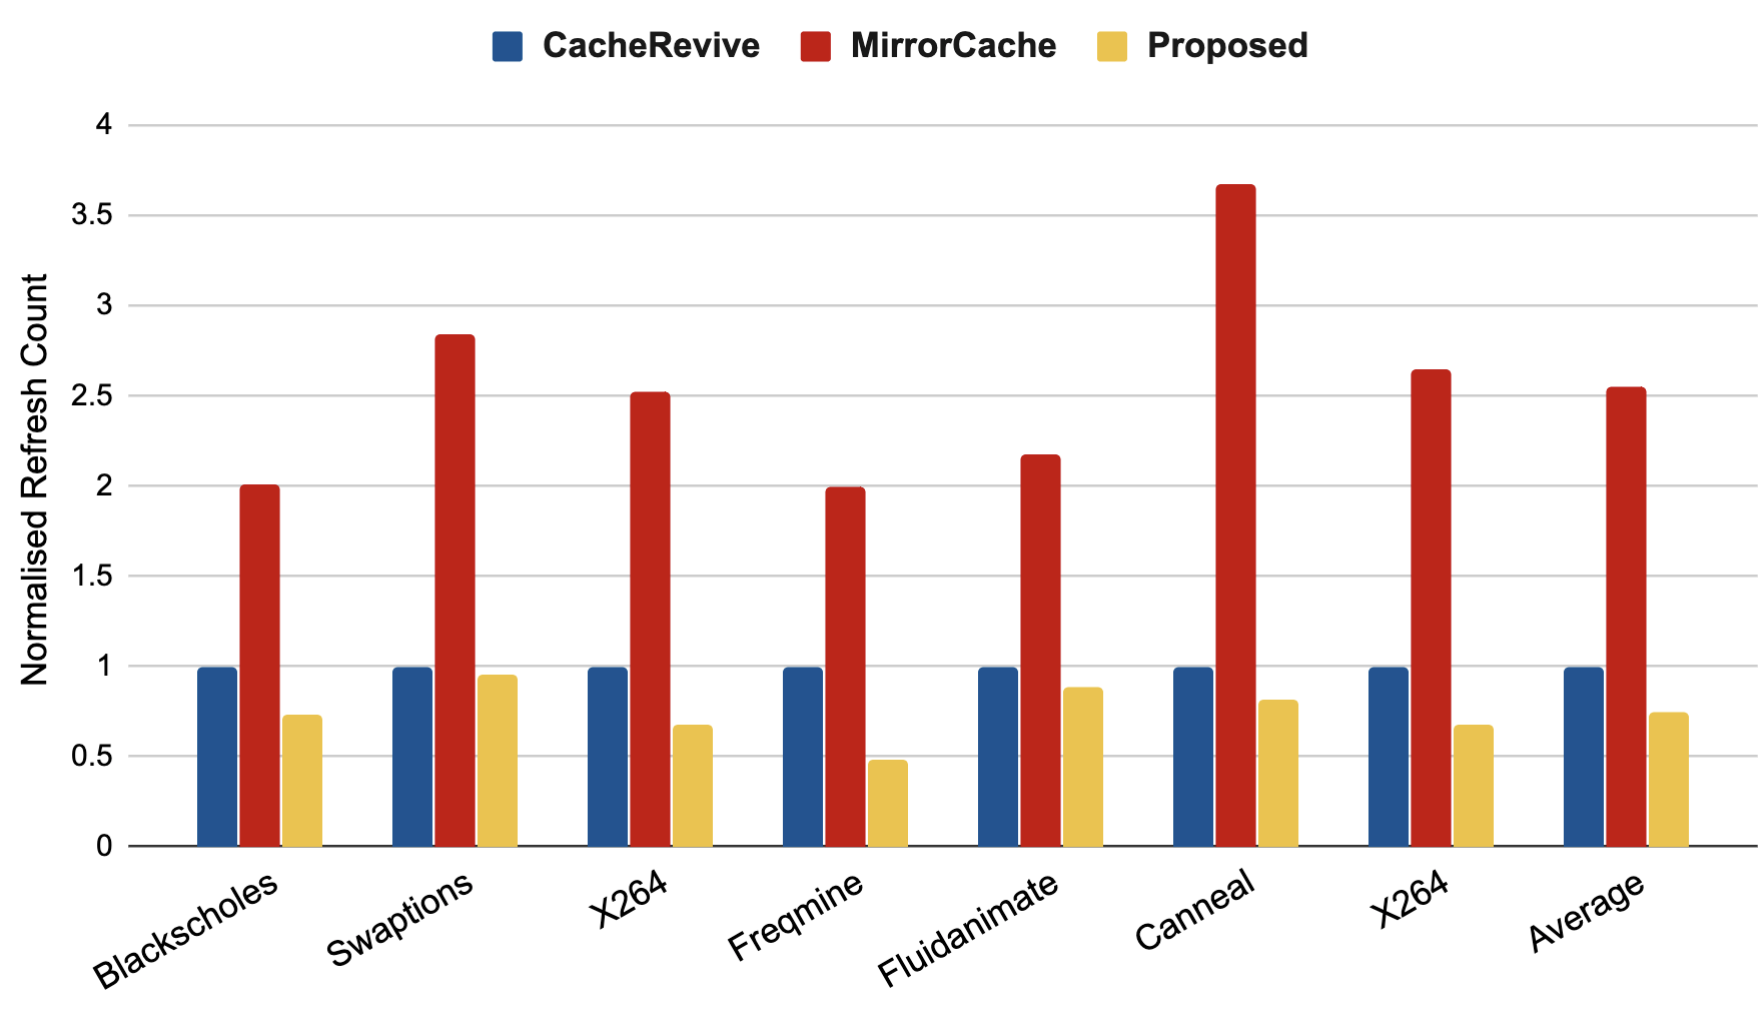
\includegraphics[width=\columnwidth]{res/ref_count.png}
\caption{Refresh count normalised to CacheRevive}
\end{figure}

\begin{figure}[th]
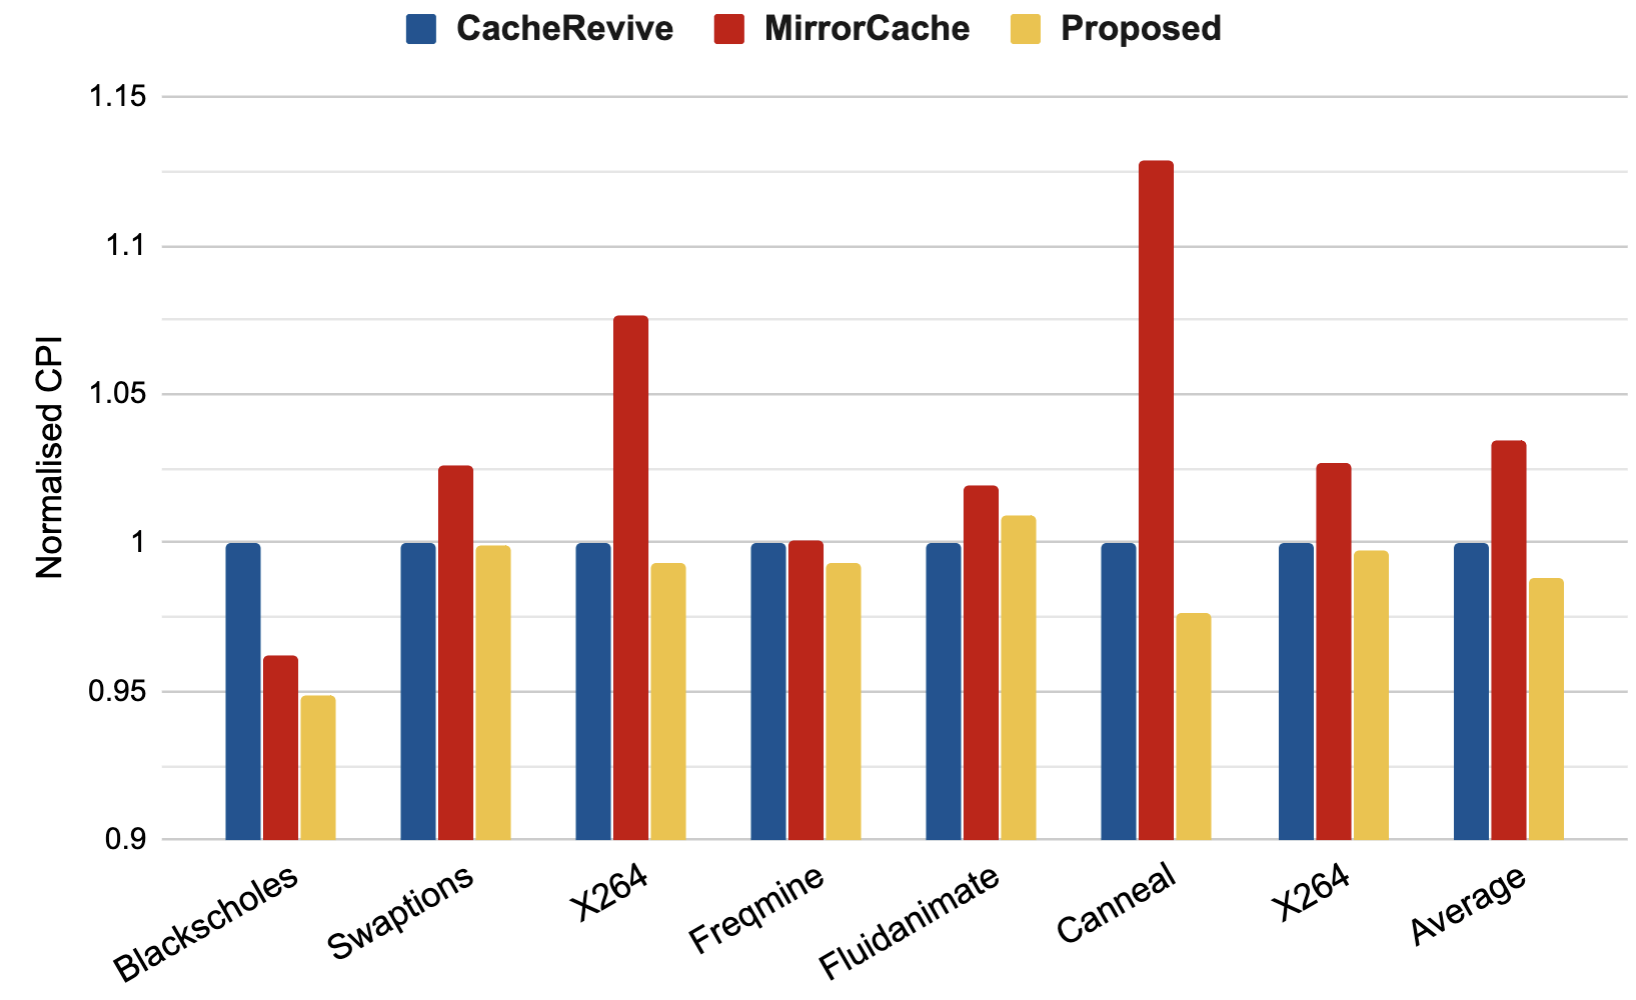
\includegraphics[width=\columnwidth]{res/cpi_perf.png}
\caption{Performance normalised to CacheRevive}
\end{figure}

\section{EXPERIMENTAL EVALUATION}
We evaluate our proposal on GEM5\cite{gem5} through full system simulation. The cache memory is modeled using ruby module and the two level MESI CMP based coherence protocol is used. We modified GEM5 to make retention time cache memory tunable. We have also implemented CacheRevive \cite{cache_revive} and MirrorCache \cite{mirror_cache} for comparison as they are the most related work to ours.

The hardware configuration uses a 2 GHz, Quad-core X86 processor. A STT-RAM based 32KB private L1 I/D (separate) cache having 64B blocks and 4-way set associativity. A SRAM based 1MB shared L2 cache with 64B block size and 16-way set associativity. Both the levels of cache use LRU and write back policy. The retention time of the STT-RAM is taken as \SI{100}{\micro\second} and \SI{1}{\milli\second} for all the simulation as the revival time of L1 cache blocks lies around this range \cite{liang}. Using the MTJ cell modeling technique in \cite{stt_ram}, we modeled the relaxed retention time STT-RAM in NVSim \cite{nvsim}. The obtained values are shown in Table 1. PARSEC \cite{parsec} benchmark suite is used in the simulations with small input set. All the overheads and changes related to dual STT-RAM read/write latency and refresh latency are taken into consideration during simulations as well.

\section{ Results and Analysis}

\textbf{Number of refreshes:} Figure 4 shows the refresh counts for MirrorCache
\begin{figure}[t]
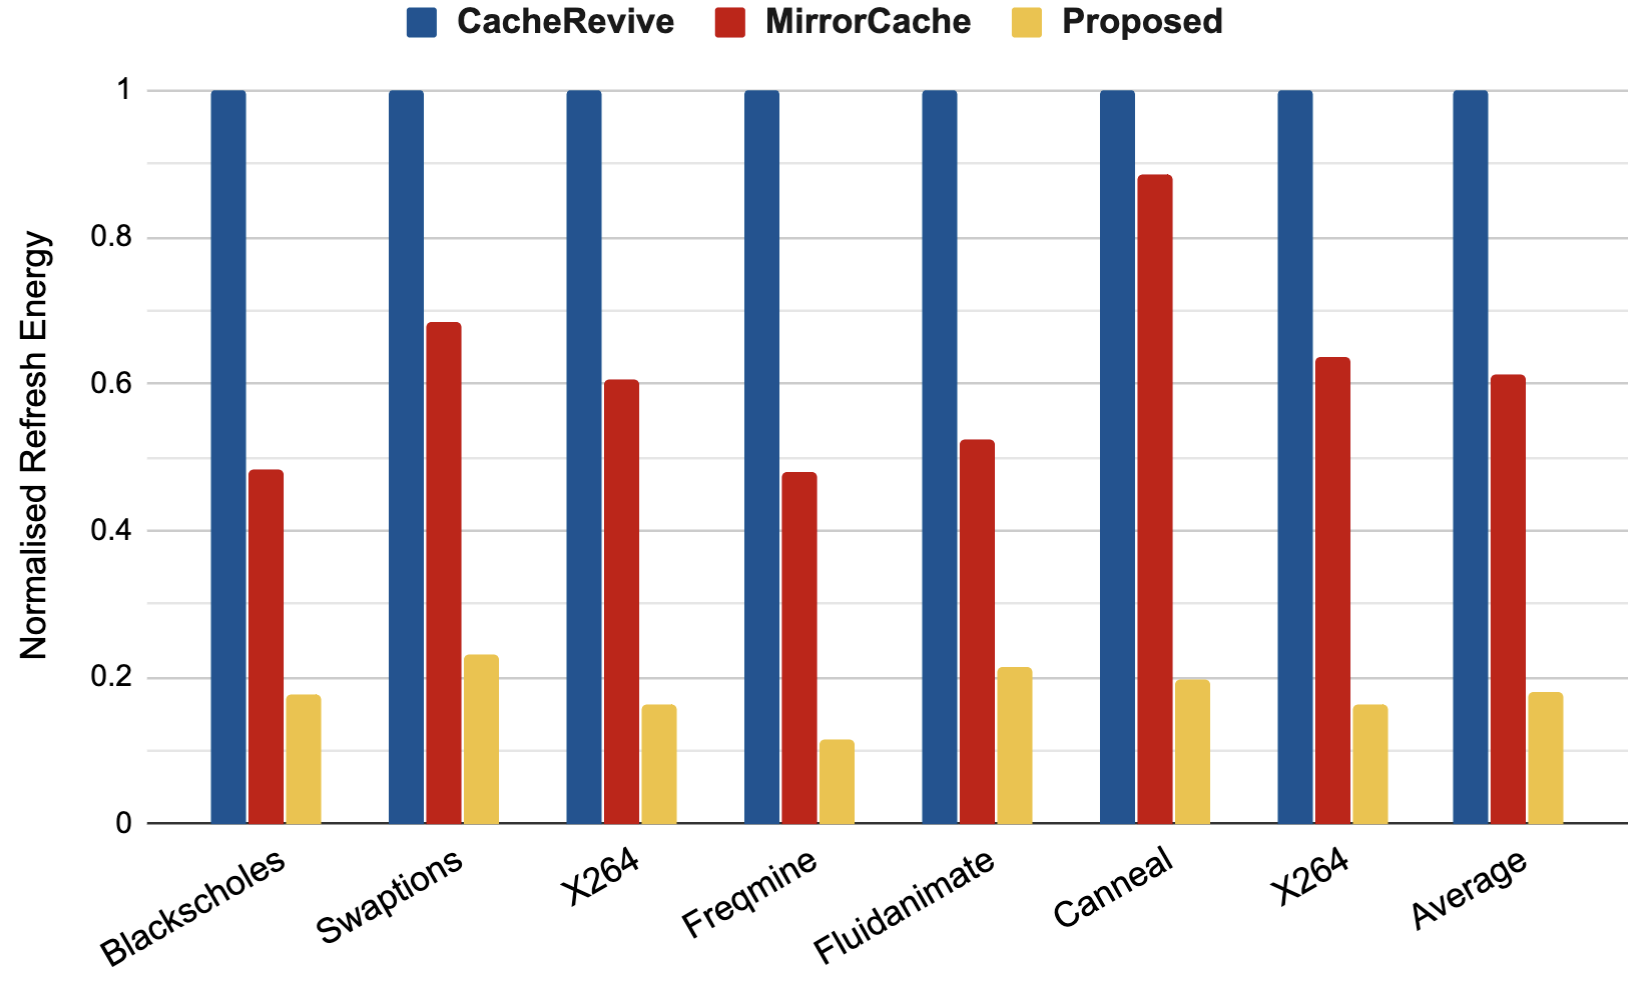
\includegraphics[width=\columnwidth]{res/ref_energy.png}
\caption{Normalised refresh energy}
\end{figure}
and our proposed method normalised to CacheRevive \cite{cache_revive}. 
We observe a significant reduction in number of refreshes by our method when compared to both the prior works. In comparison to MirrorCache, it is reduced by average of 70\% with it being atleast 55\% for every benchmark and going as high as 78\% for \textit{canneal}. On the other hand the average reduction against CacheRevive is 25\% with maximum being 51\%. The saving are higher against first method as every expiring block gets refreshed in this case while the latter already reduces its total by only choosing to top MRU blocks to refresh. By identifying the  blocks which are not resulting in further cache-hits even after being refreshed multiple times, the proposed method keeps the refresh confidence of those blocks lower which a saves significant number of refreshes. This can be seen with the benchmarks having higher non-access refreshes showing relatively larger reduction in total refresh count. Due to sizeable reduction in refreshes, the execution time of application is also reduced as there are lesser stalls during normal memory accesses which further reduces the need for a block's refresh.\vspace{1em}

\begin{figure}[t]
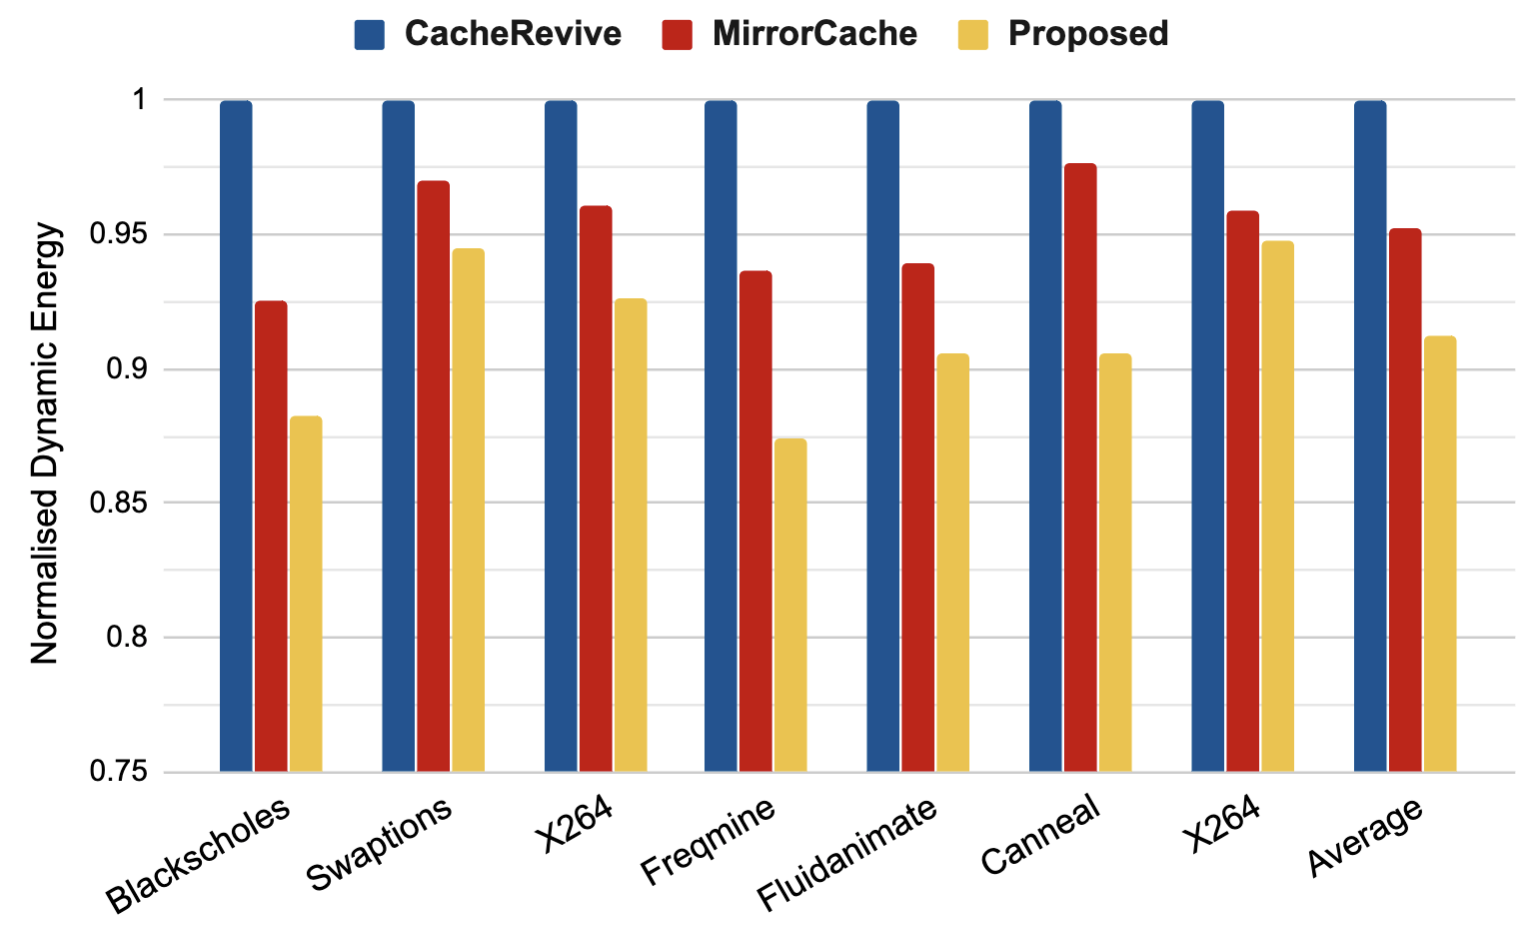
\includegraphics[width=\columnwidth]{res/dyn_energy.png}
\caption{Total dynamic energy}
\end{figure}





 \noindent \textbf{Performance: } A refresh operation positively affects performance by preventing a cache miss and negatively by stalling normal cache access operations that comes during an ongoing refresh. The net effect of these two factors affects the applications performance as a whole. Figure 5 shows the normalized Cycles Per Instruction (CPI). The proposed method improves performance by an average of 6.3\% w.r.t MirrorCache and 1.3\% w.r.t to CacheRevive. Since reducing the refreshes increases cache miss rate, the cycles saved by reduced refresh operations is counter balanced to an extent by the few cache misses having higher miss penalty. Nevertheless we are able to save significant energy on refresh with a slight performance improvement as well.\vspace{1em}


\noindent \textbf{Energy Consumption: }The reduction in refresh count directly impacts energy consumption of the cache. Total energy of the cache comprises of static energy, dynamic access energy and refresh energy. We only did a comparison on the dynamic and refresh energy as all the three methods use the same configuration of STT-RAM. Figure 6 illustrates the normalized reduction in refresh energy where our proposed method achieves an average reduction of 84\% and 71\% in comparison to CacheRevive and MirrorCache respectively. When compared to CacheRevive we are able to reduce the energy more due to the reduction in refresh count as well as reduction in refresh energy as we do not use a highly associative refresh buffer. Figure 7 shows the normalized reduction in total dynamic energy in the range of 5-12\% with an average of 9\% w.r.t CacheRevive and an average of 4\% w.r.t MirrorCache.


\section{CONCLUSION}

In this paper, we propose a refresh optimized STT-RAM based L1 cache design for mitigating the refresh overheads in existing designs that uses relaxed retention time STT-RAM. In spite of STT-RAM's multiple features like low leakage power and high density, making its write latency and energy competitive to SRAM is a crucial issue that needs to be addressed for it to be able to replace SRAM. To this end, relaxing the retention time close to the revival time of majority of blocks is a viable alternative with energy overheads either due to utilizing a refresh buffer or doing large number of refreshes. Our proposed method leverages the cache access pattern to learn refresh confidence for the blocks and a refresh threshold for the whole cache that is used to decide when to refresh the blocks. The energy saving comes from reducing the refreshes as well as using an auxiliary segment instead of a refresh buffer.
   
From experiments it was observed that refreshes were reduced by 25\% and dynamic energy was reduced by 9\% in comparison with CacheRevive. With less stalls due reduced refreshes we observe an average performance gain of 1.3\%. Thus, if we reduce the dynamic refreshes carefully without significant increase in cache misses we can save on energy and performance in already optimized STT-RAM architectures. 











% \subsection{Template Styles}

% The primary parameter given to the ``\verb|acmart|'' document class is
% the {\itshape template style} which corresponds to the kind of publication
% or SIG publishing the work. This parameter is enclosed in square
% brackets and is a part of the {\verb|documentclass|} command:
% \begin{verbatim}
%   \documentclass[STYLE]{acmart}
% \end{verbatim}

% Journals use one of three template styles. All but three ACM journals
% use the {\verb|acmsmall|} template style:
% \begin{itemize}
% \item {\verb|acmsmall|}: The default journal template style.
% \item {\verb|acmlarge|}: Used by JOCCH and TAP.
% \item {\verb|acmtog|}: Used by TOG.
% \end{itemize}

% The majority of conference proceedings documentation will use the {\verb|acmconf|} template style.
% \begin{itemize}
% \item {\verb|acmconf|}: The default proceedings template style.
% \item{\verb|sigchi|}: Used for SIGCHI conference articles.
% \item{\verb|sigchi-a|}: Used for SIGCHI ``Extended Abstract'' articles.
% \item{\verb|sigplan|}: Used for SIGPLAN conference articles.
% \end{itemize}

% \subsection{Template Parameters}

% In addition to specifying the {\itshape template style} to be used in
% formatting your work, there are a number of {\itshape template parameters}
% which modify some part of the applied template style. A complete list
% of these parameters can be found in the {\itshape \LaTeX\ User's Guide.}

% Frequently-used parameters, or combinations of parameters, include:
% \begin{itemize}
% \item {\verb|anonymous,review|}: Suitable for a ``double-blind''
%   conference submission. Anonymizes the work and includes line
%   numbers. Use with the \verb|\acmSubmissionID| command to print the
%   submission's unique ID on each page of the work.
% \item{\verb|authorversion|}: Produces a version of the work suitable
%   for posting by the author.
% \item{\verb|screen|}: Produces colored hyperlinks.
% \end{itemize}

% This document uses the following string as the first command in the
% source file:
% \begin{verbatim}
% \documentclass[sigconf]{acmart}
% \end{verbatim}

% \section{Modifications}

% Modifying the template --- including but not limited to: adjusting
% margins, typeface sizes, line spacing, paragraph and list definitions,
% and the use of the \verb|\vspace| command to manually adjust the
% vertical spacing between elements of your work --- is not allowed.

% {\bfseries Your document will be returned to you for revision if
%   modifications are discovered.}

% \section{Typefaces}

% The ``\verb|acmart|'' document class requires the use of the
% ``Libertine'' typeface family. Your \TeX\ installation should include
% this set of packages. Please do not substitute other typefaces. The
% ``\verb|lmodern|'' and ``\verb|ltimes|'' packages should not be used,
% as they will override the built-in typeface families.

% \section{Title Information}

% The title of your work should use capital letters appropriately -
% \url{https://capitalizemytitle.com/} has useful rules for
% capitalization. Use the {\verb|title|} command to define the title of
% your work. If your work has a subtitle, define it with the
% {\verb|subtitle|} command.  Do not insert line breaks in your title.

% If your title is lengthy, you must define a short version to be used
% in the page headers, to prevent overlapping text. The \verb|title|
% command has a ``short title'' parameter:
% \begin{verbatim}
%   \title[short title]{full title}
% \end{verbatim}

% \section{Authors and Affiliations}

% Each author must be defined separately for accurate metadata
% identification. Multiple authors may share one affiliation. Authors'
% names should not be abbreviated; use full first names wherever
% possible. Include authors' e-mail addresses whenever possible.

% Grouping authors' names or e-mail addresses, or providing an ``e-mail
% alias,'' as shown below, is not acceptable:
% \begin{verbatim}
%   \author{Brooke Aster, David Mehldau}
%   \email{dave,judy,steve@university.edu}
%   \email{firstname.lastname@phillips.org}
% \end{verbatim}

% The \verb|authornote| and \verb|authornotemark| commands allow a note
% to apply to multiple authors --- for example, if the first two authors
% of an article contributed equally to the work.

% If your author list is lengthy, you must define a shortened version of
% the list of authors to be used in the page headers, to prevent
% overlapping text. The following command should be placed just after
% the last \verb|\author{}| definition:
% \begin{verbatim}
%   \renewcommand{\shortauthors}{McCartney, et al.}
% \end{verbatim}
% Omitting this command will force the use of a concatenated list of all
% of the authors' names, which may result in overlapping text in the
% page headers.

% The article template's documentation, available at
% \url{https://www.acm.org/publications/proceedings-template}, has a
% complete explanation of these commands and tips for their effective
% use.

% \section{Rights Information}

% Authors of any work published by ACM will need to complete a rights
% form. Depending on the kind of work, and the rights management choice
% made by the author, this may be copyright transfer, permission,
% license, or an OA (open access) agreement.

% Regardless of the rights management choice, the author will receive a
% copy of the completed rights form once it has been submitted. This
% form contains \LaTeX\ commands that must be copied into the source
% document. When the document source is compiled, these commands and
% their parameters add formatted text to several areas of the final
% document:
% \begin{itemize}
% \item the ``ACM Reference Format'' text on the first page.
% \item the ``rights management'' text on the first page.
% \item the conference information in the page header(s).
% \end{itemize}

% Rights information is unique to the work; if you are preparing several
% works for an event, make sure to use the correct set of commands with
% each of the works.

% \section{CCS Concepts and User-Defined Keywords}

% Two elements of the ``acmart'' document class provide powerful
% taxonomic tools for you to help readers find your work in an online
% search.

% The ACM Computing Classification System ---
% \url{https://www.acm.org/publications/class-2012} --- is a set of
% classifiers and concepts that describe the computing
% discipline. Authors can select entries from this classification
% system, via \url{https://dl.acm.org/ccs/ccs.cfm}, and generate the
% commands to be included in the \LaTeX\ source.

% User-defined keywords are a comma-separated list of words and phrases
% of the authors' choosing, providing a more flexible way of describing
% the research being presented.

% CCS concepts and user-defined keywords are required for all short- and
% full-length articles, and optional for two-page abstracts.

% \section{Sectioning Commands}

% Your work should use standard \LaTeX\ sectioning commands:
% \verb|section|, \verb|subsection|, \verb|subsubsection|, and
% \verb|paragraph|. They should be numbered; do not remove the numbering
% from the commands.

% Simulating a sectioning command by setting the first word or words of
% a paragraph in boldface or italicized text is {\bfseries not allowed.}

% \section{Tables}

% The ``\verb|acmart|'' document class includes the ``\verb|booktabs|''
% package --- \url{https://ctan.org/pkg/booktabs} --- for preparing
% high-quality tables.

% Table captions are placed {\itshape above} the table.

% Because tables cannot be split across pages, the best placement for
% them is typically the top of the page nearest their initial cite.  To
% ensure this proper ``floating'' placement of tables, use the
% environment \textbf{table} to enclose the table's contents and the
% table caption.  The contents of the table itself must go in the
% \textbf{tabular} environment, to be aligned properly in rows and
% columns, with the desired horizontal and vertical rules.  Again,
% detailed instructions on \textbf{tabular} material are found in the
% \textit{\LaTeX\ User's Guide}.

% Immediately following this sentence is the point at which
% Table~\ref{tab:freq} is included in the input file; compare the
% placement of the table here with the table in the printed output of
% this document.

% \begin{table}
%   \caption{Frequency of Special Characters}
%   \label{tab:freq}
%   \begin{tabular}{ccl}
%     \toprule
%     Non-English or Math&Frequency&Comments\\
%     \midrule
%     \O & 1 in 1,000& For Swedish names\\
%     $\pi$ & 1 in 5& Common in math\\
%     \$ & 4 in 5 & Used in business\\
%     $\Psi^2_1$ & 1 in 40,000& Unexplained usage\\
%   \bottomrule
% \end{tabular}
% \end{table}

% To set a wider table, which takes up the whole width of the page's
% live area, use the environment \textbf{table*} to enclose the table's
% contents and the table caption.  As with a single-column table, this
% wide table will ``float'' to a location deemed more
% desirable. Immediately following this sentence is the point at which
% Table~\ref{tab:commands} is included in the input file; again, it is
% instructive to compare the placement of the table here with the table
% in the printed output of this document.

% \begin{table*}
%   \caption{Some Typical Commands}
%   \label{tab:commands}
%   \begin{tabular}{ccl}
%     \toprule
%     Command &A Number & Comments\\
%     \midrule
%     \texttt{{\char'134}author} & 100& Author \\
%     \texttt{{\char'134}table}& 300 & For tables\\
%     \texttt{{\char'134}table*}& 400& For wider tables\\
%     \bottomrule
%   \end{tabular}
% \end{table*}

% \section{Math Equations}
% You may want to display math equations in three distinct styles:
% inline, numbered or non-numbered display.  Each of the three are
% discussed in the next sections.

% \subsection{Inline (In-text) Equations}
% A formula that appears in the running text is called an inline or
% in-text formula.  It is produced by the \textbf{math} environment,
% which can be invoked with the usual
% \texttt{{\char'134}begin\,\ldots{\char'134}end} construction or with
% the short form \texttt{\$\,\ldots\$}. You can use any of the symbols
% and structures, from $\alpha$ to $\omega$, available in
% \LaTeX~\cite{Lamport:LaTeX}; this section will simply show a few
% examples of in-text equations in context. Notice how this equation:
% \begin{math}
%   \lim_{n\rightarrow \infty}x=0
% \end{math},
% set here in in-line math style, looks slightly different when
% set in display style.  (See next section).

% \subsection{Display Equations}
% A numbered display equation---one set off by vertical space from the
% text and centered horizontally---is produced by the \textbf{equation}
% environment. An unnumbered display equation is produced by the
% \textbf{displaymath} environment.

% Again, in either environment, you can use any of the symbols and
% structures available in \LaTeX\@; this section will just give a couple
% of examples of display equations in context.  First, consider the
% equation, shown as an inline equation above:
% \begin{equation}
%   \lim_{n\rightarrow \infty}x=0
% \end{equation}
% Notice how it is formatted somewhat differently in
% the \textbf{displaymath}
% environment.  Now, we'll enter an unnumbered equation:
% \begin{displaymath}
%   \sum_{i=0}^{\infty} x + 1
% \end{displaymath}
% and follow it with another numbered equation:
% \begin{equation}
%   \sum_{i=0}^{\infty}x_i=\int_{0}^{\pi+2} f
% \end{equation}
% just to demonstrate \LaTeX's able handling of numbering.

% \section{Figures}

% The ``\verb|figure|'' environment should be used for figures. One or
% more images can be placed within a figure. If your figure contains
% third-party material, you must clearly identify it as such, as shown
% in the example below.
% \begin{figure}[h]
%   \centering
%   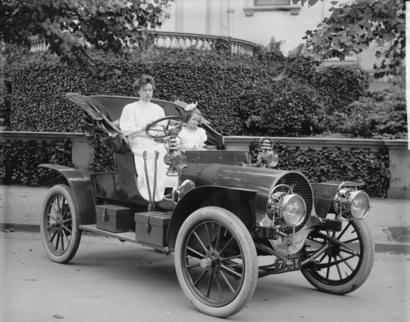
\includegraphics[width=\linewidth]{sample-franklin}
%   \caption{1907 Franklin Model D roadster. Photograph by Harris \&
%     Ewing, Inc. [Public domain], via Wikimedia
%     Commons. (\url{https://goo.gl/VLCRBB}).}
%   \Description{The 1907 Franklin Model D roadster.}
% \end{figure}

% Your figures should contain a caption which describes the figure to
% the reader. Figure captions go below the figure. Your figures should
% {\bfseries also} include a description suitable for screen readers, to
% assist the visually-challenged to better understand your work.

% Figure captions are placed {\itshape below} the figure.

% \subsection{The ``Teaser Figure''}

% A ``teaser figure'' is an image, or set of images in one figure, that
% are placed after all author and affiliation information, and before
% the body of the article, spanning the page. If you wish to have such a
% figure in your article, place the command immediately before the
% \verb|\maketitle| command:
% \begin{verbatim}
%   \begin{teaserfigure}
%     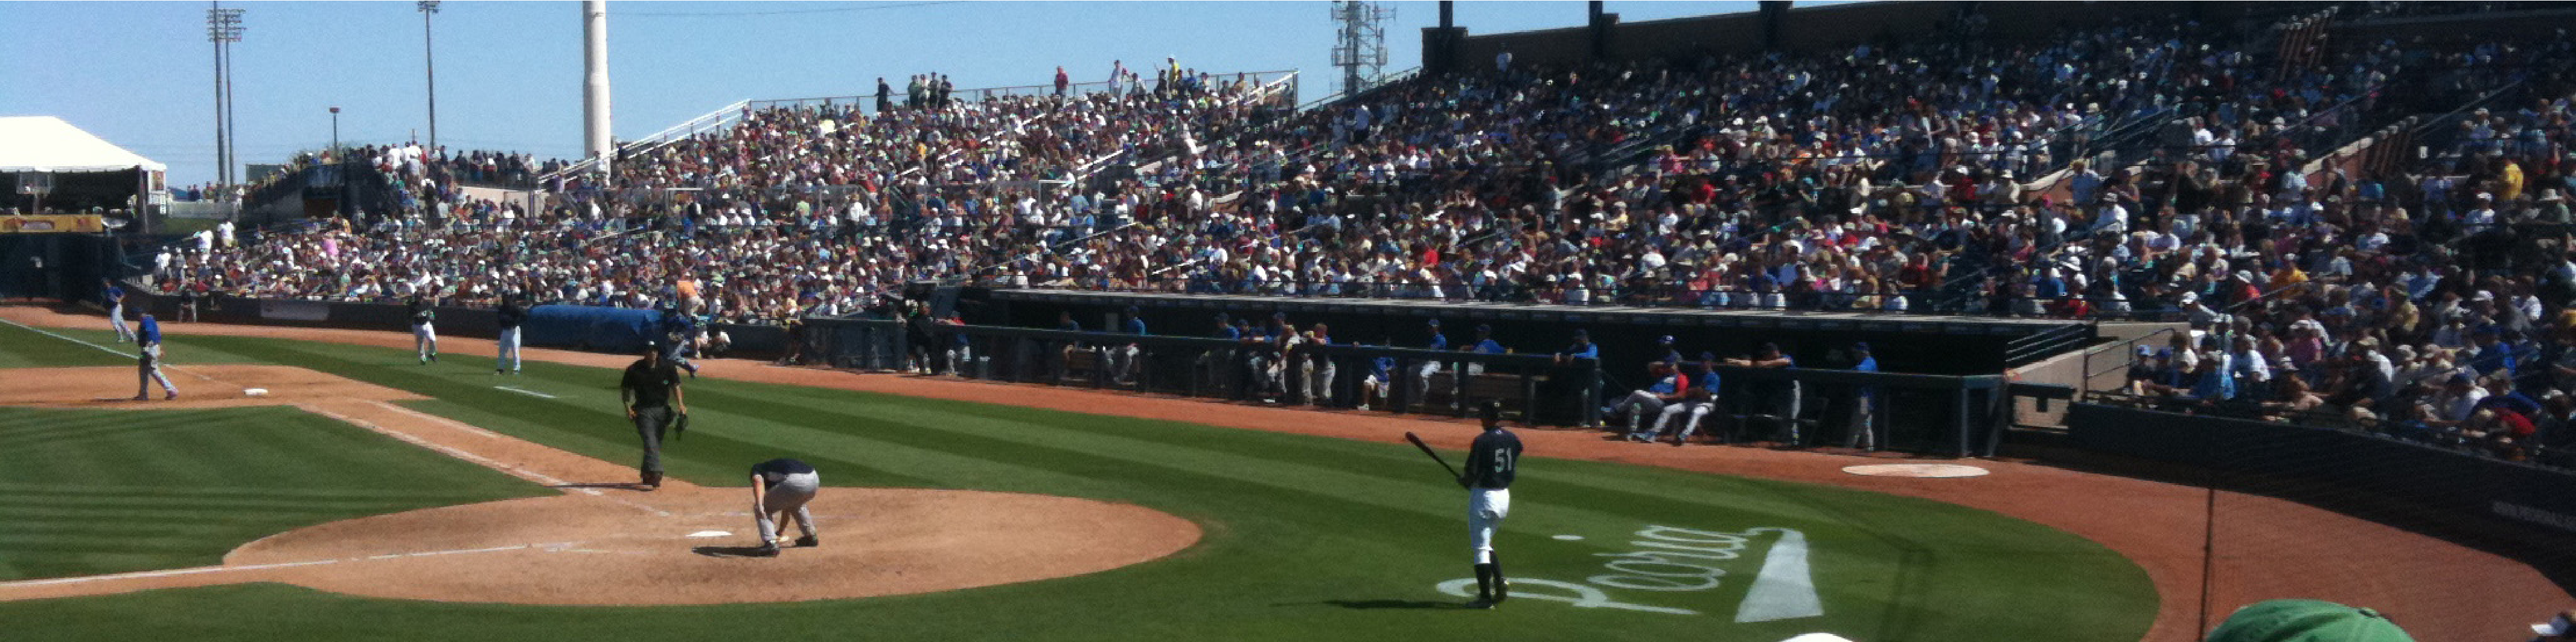
\includegraphics[width=\textwidth]{sampleteaser}
%     \caption{figure caption}
%     \Description{figure description}
%   \end{teaserfigure}
% \end{verbatim}

% \section{Citations and Bibliographies}

% The use of \BibTeX\ for the preparation and formatting of one's
% references is strongly recommended. Authors' names should be complete
% --- use full first names (``Donald E. Knuth'') not initials
% (``D. E. Knuth'') --- and the salient identifying features of a
% reference should be included: title, year, volume, number, pages,
% article DOI, etc.

% The bibliography is included in your source document with these two
% commands, placed just before the \verb|\end{document}| command:
% \begin{verbatim}
%   \bibliographystyle{ACM-Reference-Format}
%   \bibliography{bibfile}
% \end{verbatim}
% where ``\verb|bibfile|'' is the name, without the ``\verb|.bib|''
% suffix, of the \BibTeX\ file.

% Citations and references are numbered by default. A small number of
% ACM publications have citations and references formatted in the
% ``author year'' style; for these exceptions, please include this
% command in the {\bfseries preamble} (before
% ``\verb|\begin{document}|'') of your \LaTeX\ source:
% \begin{verbatim}
%   \citestyle{acmauthoryear}
% \end{verbatim}

%   Some examples.  A paginated journal article \cite{test}, an
%   enumerated journal article \cite{Cohen07}, a reference to an entire
%   issue \cite{JCohen96}, a monograph (whole book) \cite{Kosiur01}, a
%   monograph/whole book in a series (see 2a in spec. document)
%   \cite{Harel79}, a divisible-book such as an anthology or compilation
%   \cite{Editor00} followed by the same example, however we only output
%   the series if the volume number is given \cite{Editor00a} (so
%   Editor00a's series should NOT be present since it has no vol. no.),
%   a chapter in a divisible book \cite{Spector90}, a chapter in a
%   divisible book in a series \cite{Douglass98}, a multi-volume work as
%   book \cite{Knuth97}, an article in a proceedings (of a conference,
%   symposium, workshop for example) (paginated proceedings article)
%   \cite{Andler79}, a proceedings article with all possible elements
%   \cite{Smith10}, an example of an enumerated proceedings article
%   \cite{VanGundy07}, an informally published work \cite{Harel78}, a
%   doctoral dissertation \cite{Clarkson85}, a master's thesis:
%   \cite{anisi03}, an online document / world wide web resource
%   \cite{Thornburg01, Ablamowicz07, Poker06}, a video game (Case 1)
%   \cite{Obama08} and (Case 2) \cite{Novak03} and \cite{Lee05} and
%   (Case 3) a patent \cite{JoeScientist001}, work accepted for
%   publication \cite{rous08}, 'YYYYb'-test for prolific author
%   \cite{SaeediMEJ10} and \cite{SaeediJETC10}. Other cites might
%   contain 'duplicate' DOI and URLs (some SIAM articles)
%   \cite{Kirschmer:2010:AEI:1958016.1958018}. Boris / Barbara Beeton:
%   multi-volume works as books \cite{MR781536} and \cite{MR781537}. A
%   couple of citations with DOIs:
%   \cite{2004:ITE:1009386.1010128,Kirschmer:2010:AEI:1958016.1958018}. Online
%   citations: \cite{TUGInstmem, Thornburg01, CTANacmart}. Artifacts:
%   \cite{R} and \cite{UMassCitations}.

% \section{Acknowledgments}

% Identification of funding sources and other support, and thanks to
% individuals and groups that assisted in the research and the
% preparation of the work should be included in an acknowledgment
% section, which is placed just before the reference section in your
% document.

% This section has a special environment:
% \begin{verbatim}
%   \begin{acks}
%   ...
%   \end{acks}
% \end{verbatim}
% so that the information contained therein can be more easily collected
% during the article metadata extraction phase, and to ensure
% consistency in the spelling of the section heading.

% Authors should not prepare this section as a numbered or unnumbered {\verb|\section|}; please use the ``{\verb|acks|}'' environment.

% \section{Appendices}

% If your work needs an appendix, add it before the
% ``\verb|\end{document}|'' command at the conclusion of your source
% document.

% Start the appendix with the ``\verb|appendix|'' command:
% \begin{verbatim}
%   \appendix
% \end{verbatim}
% and note that in the appendix, sections are lettered, not
% numbered. This document has two appendices, demonstrating the section
% and subsection identification method.

% \section{SIGCHI Extended Abstracts}

% The ``\verb|sigchi-a|'' template style (available only in \LaTeX\ and
% not in Word) produces a landscape-orientation formatted article, with
% a wide left margin. Three environments are available for use with the
% ``\verb|sigchi-a|'' template style, and produce formatted output in
% the margin:
% \begin{itemize}
% \item {\verb|sidebar|}:  Place formatted text in the margin.
% \item {\verb|marginfigure|}: Place a figure in the margin.
% \item {\verb|margintable|}: Place a table in the margin.
% \end{itemize}

%%
%% The acknowledgments section is defined using the "acks" environment
%% (and NOT an unnumbered section). This ensures the proper
%% identification of the section in the article metadata, and the
%% consistent spelling of the heading.
% \begin{acks}
% To Robert, for the bagels and explaining CMYK and color spaces.
% \end{acks}

%%
%% The next two lines define the bibliography style to be used, and
%% the bibliography file.
\bibliographystyle{ACM-Reference-Format}
\bibliography{sample-base}

%%
%% If your work has an appendix, this is the place to put it.


\end{document}
\endinput
%%
%% End of file `sample-sigconf.tex'.
